\chapter{ベストセラー小説を書くには}

この講義は、私たちをいったん誤った方向へ誘惑するところから始まる。書斎、隠し扉、本棚、本が生まれる場所が示される。そしてすぐに、その誘惑は取り下げられる。airport lounge でも、plane の中でも、car の中でも書けるのだ、と。lesson は room ではない。process である。そこから interview は、互いに linked した problems の sequence として unfold する。information はどう arrange されるのか、comments はどう diagnoses になるのか、なぜ revision は recomposition として扱われるのか、その recomposition にはどれほどの時間がかかるのか、そして長大な manuscript が突然 unreadable に見え始めたとき、何をするのか、という sequence である。

\section{room、そして method への swift な turn}

opening が useful なのは、まさにそれが一瞬 misleading だからである。私たちは place から始める。だが講師は、place に explanatory weight を carry させることを refuse する。書斎は pleasant である。ひょっとすると best place ですらあるかもしれない。だが writing は、他のどこででも起こりうる、と私たちは told される。これによって本当の subject のための ground が clear される。ambience ではなく、method である。

この最初の turn は重要である。weaker な lecture なら、writerly atmosphere の level に remain していただろう。この lecture はそうしない。room を entry として扱い、process を substance として扱う。したがって私たちは、ほとんど immediately に、本当の pivot に備えさせられる。three-screen setup と、novel が draft から draft へ move する mechanics である。

\subsection{Question \& Answer}

\paragraph{Question.} writer に必要なのは ideal な room なのか、それとも working process だけなのか。

\paragraph{Answer.} この講義の答えでは、よい room は helpful ではあるが decisive ではない。matter するのは repeatable な process である。room は work を support するかもしれないが、work を explain はしない。

\section{three screens と revision の flow}

room が demoted されると、interview は technical になる。mood ではなく process が示されるのである。one screen には first draft がある。another には、その draft を読んだ readers からの comments がある。middle には、進行中の second draft が sit している。この arrangement は、map として十分に simple に書ける。
\begin{equation}
\text{first draft} \to \text{reader comments} \to \text{second draft}.
\end{equation}
これが、この講義の最初の本当の mathematical spine である。そこに言われているのは、writing とは mere な production であり、そのあとに vague な reflection が続くものではない、ということだ。response を通って reconstruction へと至る、controlled な material の flow なのである。

同じ point は、第二の仕方で sharpen できる。
\begin{equation}
\text{reader response} \to \text{diagnosis} \to \text{revision priority}.
\end{equation}
comment が important なのは、merely それが uttered されたからではない。それが manuscript が actual に reader に何を doing しているかを reveal するとき、重要になるのである。

\begin{definition}
\emph{revision priority} とは、merely local な preference ではなく、structural な weakness を identify しているために、top に rise してくる comment または diagnosis のことである。
\end{definition}

monitor layout に関する validated な visual evidence は残っていないので、私たちはこの arrangement を pictorially ではなく schematically に記録する。

\begin{figure}[h]
\centering
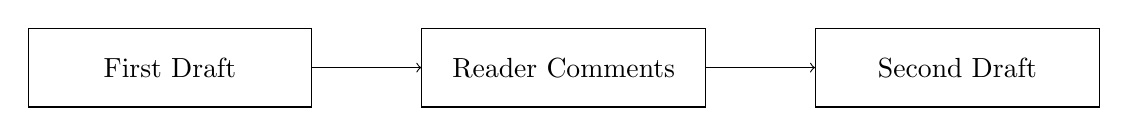
\begin{tikzpicture}
\node[draw, rectangle, minimum width=3.6cm, minimum height=1cm] (A) at (0,0) {First Draft};
\node[draw, rectangle, minimum width=3.6cm, minimum height=1cm] (B) at (5,0) {Reader Comments};
\node[draw, rectangle, minimum width=3.6cm, minimum height=1cm] (C) at (10,0) {Second Draft};
\draw[->] (A) -- (B);
\draw[->] (B) -- (C);
\end{tikzpicture}
\end{figure}

この reconstruction が deliberately minimal なのは、そのためである。この講義が equipement の fetish を与えているのではないからだ。そこに示されているのは workflow である。draft は exposed され、responses は collected され、next draft は learned ことの pressure の下で written されるのである。

\subsection{Question \& Answer}

\paragraph{Question.} revising のあいだ、writer の目の前には何の information があるべきなのか。

\paragraph{Answer.} この講義の答えは exact である。current draft、それが produce した responses、そして next draft が composed されつつある space である。これらが explicit な relation の中に hold されるとき、revision は clearer になる。

\section{comment から diagnosis へ: pace は measurable な craft problem}

講義はそのあと、この system が operation しているところを示す。ある reader は、新しい book には last two ほど quickly には drawn in されず、同じ速さでは read できなかったと言う。Follett はこれを injury として take しない。data として take する。inference は immediate である。
\begin{equation}
\text{not drawn in quickly} \Rightarrow \text{opening chapter may be ponderous}.
\end{equation}
これは craft reasoning の model act である。surface の comment が、structural problem へ translate されるのである。

その problem は、それから Follett が explicitly に述べる pacing heuristic と compare される。
\begin{equation}
\text{plot twist interval} \approx 3\text{--}4 \ \text{pages}.
\end{equation}
この rule は、fiction の universal theorem として presented されるのではない。narrative pull の working measure として presented されるのである。もし opening が十分な頻度で turning していないなら、reader の slower engagement は mystery ではない。

\paragraph{Worked example.} この reasoning は、steps にして書ける。
\begin{enumerate}
\item ある reader が、drawn in されるのが遅すぎたと report する。
\item writer は、それを personal slight として hear することを refuse する。
\item その report は structural hypothesis に translate される。opening が ponderous なのかもしれない、という仮説である。
\item その hypothesis は pacing heuristic に against して test される。
\item したがって、その comment は high revision priority へ rise する。
\end{enumerate}

interviewer はそこで necessary な question を ask する。established writer であれば、こういう comment は simply dismiss してしまうのではないか、と。その answer は、もう一つの compact relation を与える。
\begin{equation}
\text{feedback} \neq \text{insult}, \qquad
\text{feedback} \Rightarrow \text{what can I learn?}
\end{equation}
この equation は重要である。これなしには、whole three-screen system は vanity へ collapse してしまう。それがあることによって、response は affront ではなく instrument になる。

\subsection{Question \& Answer}

\paragraph{Question.} comment は、どうやって structural diagnosis になるのか。

\paragraph{Answer.} reaction から craft language へ convert されることによってである。``I was not drawn in quickly'' は taste judgment ではなく、pace に関する statement になり、そして revision の target になるのである。

\section{second draft は recomposition である}

講義の strongest claim は次に来る。Follett は second draft に move するとき、first draft を take して merely alter するのではないと言う。ordinary な sense で edit するのではない。book をもう一度 type し直すのだ。この distinction は、formal statement に値するほど strong である。
\begin{equation}
\text{second draft} \neq \text{annotated first draft}, \qquad
\text{second draft} = \text{book rewritten from scratch}.
\end{equation}
これは routine advice about revision よりも more radical である。second draft は、first object の corrected version ではない。better information のもとで produce される new construction なのである。

だからこそ center にある process screen がそれほど matter する。その center は、mere な repair の site ではない。book が again made される place なのである。comments と earlier pages は guides ではあるが、cosmetically improved されている thing そのものではない。

\subsection{Question \& Answer}

\paragraph{Question.} first draft を simply editing する instead of、なぜ whole book を rewrite するのか。

\paragraph{Answer.} この見方では、first draft はまだ proper object of polish ではないからである。それは material であり、evidence であり、diagnosis の occasion である。second draft は、higher standards と clearer understanding のもとで、book が rebuilt される場所なのだ。

\begin{remark}
この講義はこれを Follett の method と conviction として present している。それは interview の中での strong な working standard として preserve されるべきであって、すべての fiction writing に対する universal law に inflated されるべきではない。
\end{remark}

\section{long novel の arithmetic}

method が stated されると、interviewer は natural な objection を raise する。これでは longer に take するに違いない。Follett の answer は evasive ではない。arithmetic である。
\begin{equation}
\text{planning} = 1\ \text{year}, \qquad
\text{first draft} = 1\ \text{year}, \qquad
\text{second draft} = 1\ \text{year}.
\end{equation}
したがって implied な project horizon は、
\begin{equation}
T_{\text{book}} = T_{\text{plan}} + T_{\text{draft1}} + T_{\text{draft2}}.
\end{equation}
となる。これは、この講義の cleanest な contributions の一つである。novels take time する、という vague な sense を、decomposed な temporal structure へ turn してくれるからだ。

次の challenge は naturally follow する。もし second draft がそれほど much を cost するなら、それは really essential なのか。Follett の answer は yes である。publishers は sometimes first draft を publish したがるかもしれない。だが彼の view では、それは lower standard を reflect している。彼自身の conclusion は、
\begin{equation}
\text{rewrite from scratch} \Rightarrow \text{better product}.
\end{equation}
と書ける。これも again、lecture に local な statement であって universal metaphysics ではない。だが interview の logic にとって central である。time-cost は、resulting な book が better だから justify されるのである。

第二の transcript-based schematic も、ここで useful である。

\begin{figure}[h]
\centering
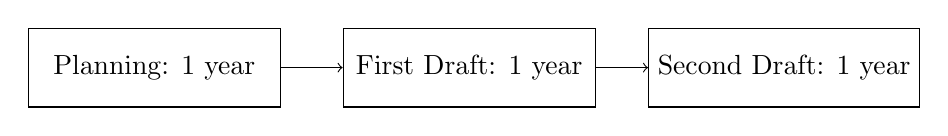
\begin{tikzpicture}
\node[draw, rectangle, minimum width=3.2cm, minimum height=1cm] (P) at (0,0) {Planning: 1 year};
\node[draw, rectangle, minimum width=3.2cm, minimum height=1cm] (F) at (4,0) {First Draft: 1 year};
\node[draw, rectangle, minimum width=3.2cm, minimum height=1cm] (S) at (8,0) {Second Draft: 1 year};
\draw[->] (P) -- (F);
\draw[->] (F) -- (S);
\end{tikzpicture}
\end{figure}

この figure の point は decoration ではない。この講義が quality を、一つの inspiration の act に concentrated されたものとしてではなく、stages に distributed されたものとして treat していることを plain にするのである。

\section{middle に訪れる severe doubt と、continuing のための rule}

講義はここで inward に pivot する。interviewer は angst、writer's block、crisis について ask する。Follett は tortured soul の grand language を refuse する。だが difficulty そのものは deny しない。代わりに、彼は every book の中で recurring に現れる moment に name を与える。manuscript の deep に入り込み、several hundred pages が written され、そこで suddenly、なぜ anybody がこれを want to read するのだろうか、という thought が come するのである。

この moment は、
\begin{equation}
\text{hundreds of pages written} \Rightarrow \text{severe doubt}.
\end{equation}
と表せる。この講義の force は、その next に何が happen するかにある。answer は revelation でも self-expression でも panic でもない。operational である。
\begin{align}
\text{doubt} &\Rightarrow \text{press on} \Rightarrow \text{rewrite later if needed},\\
\text{if draft is not good enough} &\Rightarrow \text{rewrite} \Rightarrow \text{improvement}.
\end{align}
これは、おそらくこの講義でもっとも practical な theorem である。psychological collapse は、procedural trust によって resolve される。人は stop して feeling に rule を allow しない。revision が exist するという knowledge に protected されつつ、continue するのである。

\subsection{Question \& Answer}

\paragraph{Question.} book が suddenly に its own author に unreadable に seem するとき、私たちは何をすべきか。

\paragraph{Answer.} この講義の answer は deliberately unspectacular である。continue せよ。その thought を脇へ置き、目の前の work を finish し、later に revision が judgment を pass することを trust せよ。unreadability の feeling には final authority は granted されない。

\section{standards、absorption、そして work への love}

lecture は doubt と endurance のところで end していてもおかしくなかった。だがそうしない。より strong な resolution を choose する。Follett は、writer としての自分の problem は、tortured soul ではないことだ、と人に言われたことを recall する。彼は process を love している。そこに absorbed されている。この closing relation は trivial ではない。
\begin{equation}
\text{absorption in work} \Rightarrow \text{endurance of process}.
\end{equation}
これが、それ以前のすべてを clarify する。three screens、full rewrite、three-year structure、middle of doubt で stop することの refusal。これらはすべて、work が merely tolerated されているのではなく、adored されているがゆえに sustained されうるのである。

そしてこれはまた、lecture をその hidden opening contrast に back させる。magic の source は決して room ではなかった。method だったのだ。そして method が livable に remain するのは、それが grim self-punishment ではなく attachment に animated されているからなのである。

\section{まとめ}

この lecture は、一つずつの romance を method へ turn していくことによって advance する。まず den から始め、しかし room を secret として treat することを refuse する。ついで three-screen workflow へ move し、drafting、feedback、rewriting が visible な process に organize される。single な reader comment は、pace の diagnosis へ translate され、ついで three to four pages ごとに twist があるという heuristic に against して measured される。revision はそこで redefined される。second draft は annotated first draft ではなく、from scratch に rewritten される new book なのである。この standard の arithmetic は、planning、first draft、second draft の one-year decomposition によって explicit になる。最後に lecture は、several hundred pages のあとで appear する severe doubt に face し、revision への trust に backed された continuation の rule をもって answer する。その closing note は、method 自体と同じくらい matter する。rigor が sustainable であるのは、work が loved されているからなのだ。